\chapter{Практическая часть}

\section{Процесс работы с системой}

Процесс взаимодействия с программой выглядит следующим образом:
\begin{enumerate}
    \item обученная на десятках гигабайт текста и хорошо моделирующая распределение слов в русском языке нейронная сеть дообучается на требуемом наборе данных, подстраиваясь под требуемую предметную область,
    \item \label{p2} в дообученную языковую модель подаётся затравка --- начало текста, которое модели необходимо продолжить,
    \item \label{p3} пользователь оценивает результат генерации и может вручную отредактировать или отменить его,
    \item процесс повторяется, начиная с пункта \ref*{p2}, но в качестве затравки теперь выступает результат коррекции из пункта \ref*{p3}.
\end{enumerate}

Более наглядно процесс работы продемонстрирован на рисунке \ref*{fig:pipeline}.

\begin{figure}
    \centering
    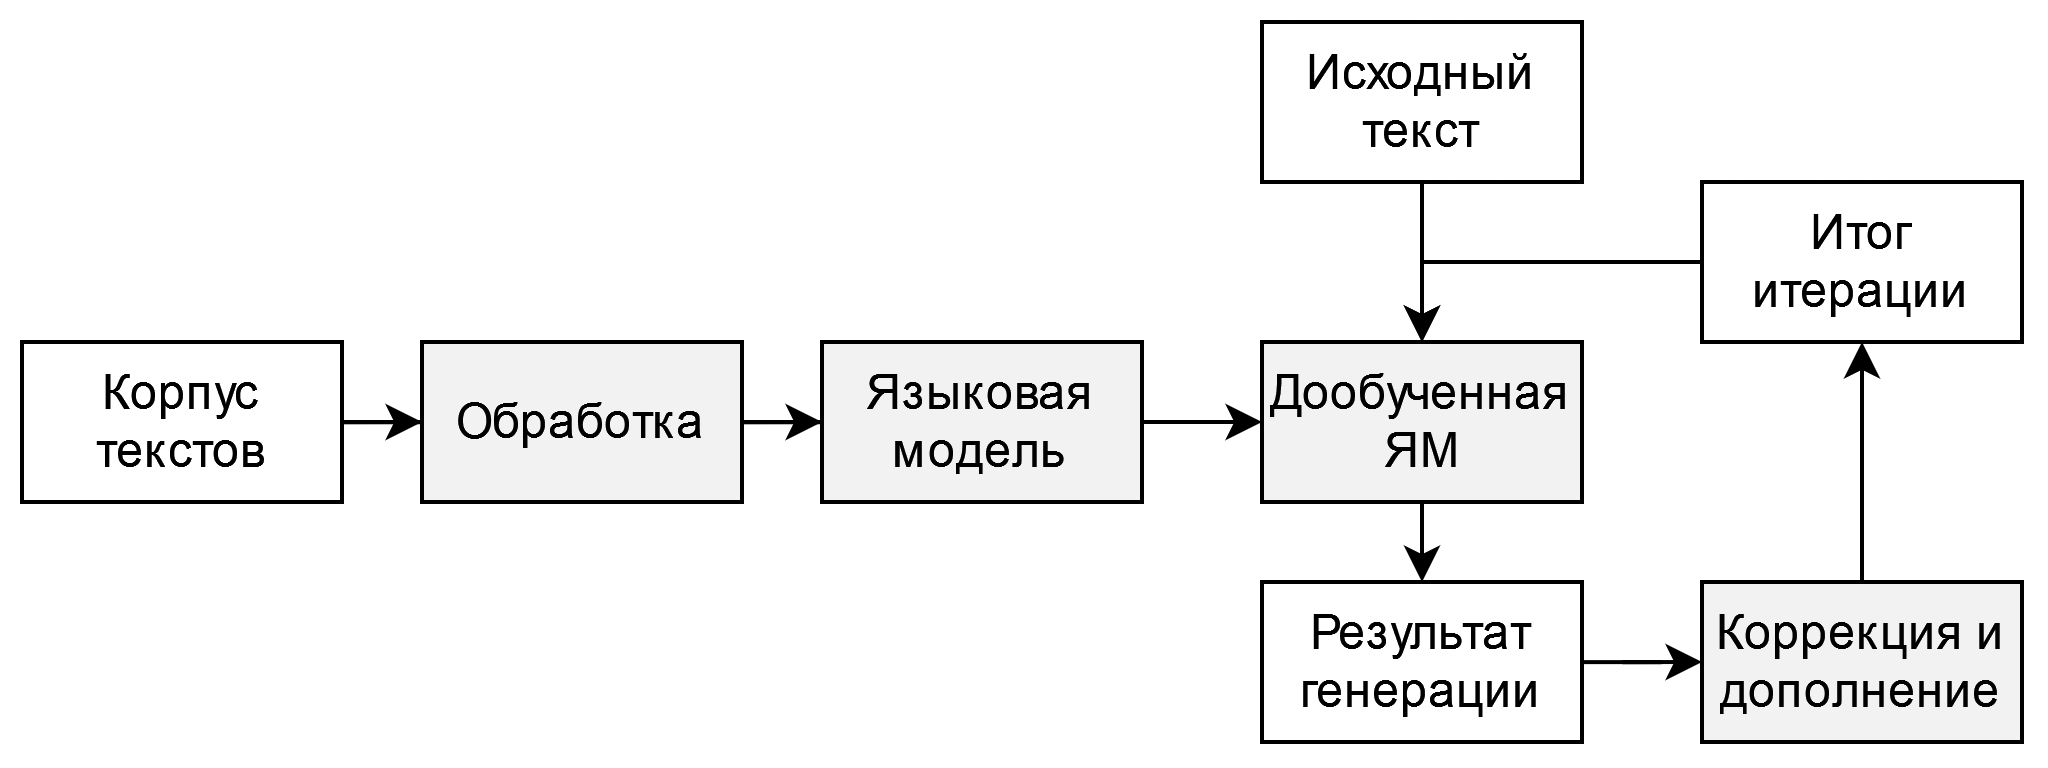
\includegraphics[width=\textwidth]{../inc/images/pipeline.png}
    \caption{Высокоуровневая схема системы}
    \label{fig:pipeline}
\end{figure}

\section{Выбор языковой модели}

Среди доступных под свободными лицензиями языковых моделей рассматривались те, что приведены в таблице \ref*{tab:models}. Они построены на основе архитектуры Transformer, показывающей лучшие на данный момент результаты в задаче генерации текста \cite{art:models_review}, а длина контекста, который они учитывают, достаточно большая, что важно для поддержания связности повествования в сгенерированном тексте. Названия моделей и их характеристики приведены в таблице \ref*{tab:models}.

\begin{table}[]
\caption{Некоторые нейросетевые языковые модели под свободными лицензиями}
\begin{tabular}{|l|l|l|l|}
\hline
Семейство модели               & Название модели & Число параметров & Длина контекста \\ \hline
\multirow{3}{*}{Russian GPT-3} & ruGPT-3 Small   & 117 млн.         & 2048            \\ \cline{2-4} 
                                & ruGPT-3 Large   & 760 млн.         & 2048            \\ \cline{2-4} 
                                & ruGPT-3 XL      & 1,3 млрд.        & 2048            \\ \hline
\multirow{3}{*}{GPT-2}         & GPT-2 Small     & 124 млн.         & 1024            \\ \cline{2-4} 
                                & GPT-2 Medium    & 355 млн.         & 1024            \\ \cline{2-4} 
                                & GPT-2 XL        & 1,5 млрд.        & 1024            \\ \hline
\end{tabular}
\label{tab:models}
\end{table}

Из рассмотренных вариантов лучшие всего подошла модель ruGPT-3 Small от <<Сбера>> \cite{art:sber_pr}. Её преимуществом является то, что она обучалась на русскоязычном корпусе и заточена под генерацию текста, в первую очередь, на русском языке, а малое относительно других моделей семейства ruGPT-3 число параметров позволяет дообучать её, располагая сравнительно небольшими мощностями.

\section{Обработка текста}

Перед обучением нейронной сети требуется привести данные к особому виду. В данном случае предварительная обработка корпуса заключается в выделении структурных блоков текста специальными синтаксическими конструкциями на естественном языке, формат которых определён заранее и сохраняется неизменным во всём корпусе. Выбор естественного языка обусловлен тем, что обученной на корпусе текстов на естественном языке языковой модели в этом случае не понадобится много данных для подстройки под новый синтаксис.

Код преобразования данных к нужному виду представлен в листинге \ref*{lst:generate}.

Пример обработанных данных показан в листинге \ref*{lst:data_sample}.

\begin{listing}[H]
\begin{verbatim}
Место действия -- ПАВ. лобби/лифт. 
Время действия -- день. день 1. 
Действующие лица -- элеонора, Управляющий, массовка. 
Ремарка -- Лифт открывается. Элеонора в лифте с букетом в руках,
дочитывает записку. Смена плана. Перед лифтом стоит Управляющий. 
Управляющий говорит: «Доброе утро, Элеонора Андреевна! Красивые
цветы!»
Элеонора говорит: «Спасибо, я и сама заметила. Ты что-то хотел?» 
Управляющий говорит: «Да. Лифт» 
Ремарка -- Элеонора выходит из лифта. Управляющий, проводив её
взглядом, входит. зк 
Макс говорит: «И вот, спустя пару недель, она явно испытывает
симпатию. Но пока к нему – незнакомцу, а не к тебе» 
Ремарка -- Лифт закрывается. 
\end{verbatim}
\caption{Пример обработанного текста}
\label{lst:data_sample}
\end{listing}

\section{Разбиение корпуса}

При обучении данные разбиваются на части, способные поместиться в видеопамять, следовательно, важно производить разбиение определённым образом для лучшего результата. Все тексты обучающей выборки разделяются на части такого размера, чтобы:
\begin{enumerate}
    \item в токенизированном виде их длина была не меньше длины контекста модели, чтобы при генерации учитывалось максимально возможное количество информации,
    \item их длина была не слишком большой, чтобы при обучении иметь возможность подавать их в модель в случайном порядке для более эффективной оптимизации,
    \item каждая часть была самостоятельным текстом, принадлежащим исходной предметной области.
\end{enumerate}

Для подачи разбитых данных в модель был написан собственный класс \Code{TextsDataset}, представленный в листинге \ref*{lst:dataset}. Он представляет собой коллекцию, которая при инициализации загружает с диска данные в виде длинных текстовых файлов, разбивает их вышеописанным способом и предоставляет интерфейс для доступа к получившимся коротким фрагментам.

\begin{lstlisting}[language=Python, caption={Класс датасета, хранящий данные в разбитом виде}, label=lst:dataset]
class TextsDataset(Dataset):
    """Texts one by one"""

    def __init__(self, tokenizer: PreTrainedTokenizer, path: str, block_size=2048):
        assert os.path.isdir(path)

        block_size = block_size - (tokenizer.max_len - tokenizer.max_len_single_sentence)

        logger.info("Creating features from dataset file at %s", path)

        self.examples = []
        try:
            for file in os.listdir(path):
                file_path = os.path.join(path, file)
                with open(file_path, encoding="utf-8") as f:
                    text = f.read()

                tokenized_text = tokenizer.convert_tokens_to_ids(tokenizer.tokenize(text))
                
                logger.info(f"Tokenized {file_path}: tokens len: {len(tokenized_text)}")

                for i in range(0, len(tokenized_text) - block_size + 1, block_size):  # Truncate in block of block_size
                    self.examples.append(
                        tokenizer.build_inputs_with_special_tokens(
                            tokenized_text[i: i + block_size]
                        )
                    )
        except Exception as e:
            logger.exception(e)
        
        logger.info(f"Created dataset of size {len(self.examples)}")

    def __len__(self):
        return len(self.examples)

    def __getitem__(self, item):
        return torch.tensor(self.examples[item], dtype=torch.long)
\end{lstlisting}

\section{Процесс обучения}

Исходная модель ruGPT-3 Small была загружена из библиотеки Transformers для языка Python. Обучение производилось с помощью оригинального программного кода от <<Сбера>> \cite{gh:sber}, в котором был изменён механизм подачи данных в модель так, чтобы это происходило с использованием собственного класса \Code{TextsDataset} из листинга \ref*{lst:dataset}.

Обучение происходило с помошью метода оптимизации Adam с шагом градиентного спуска 5∙10\textsuperscript{-5} в течение 100 эпох. В качестве набора данных были взяты сценарии юмористических телешоу. Итоговое значение перплексии составило 10,7.

\section{Пользовательский интерфейс}

Для создания графического интерфейса пользователя был использован фреймворк Streamlit. Он позволяет средствами языка Python создавать веб-приложения, которые открываются прямо в браузере на любой операционной системе \cite{doc:streamlit}.

Пользователь взаимодействует с программой через следующие элементы управления:
\begin{itemize}
    \item поле ввода текста,
    \item кнопка <<Дополнить>>,
    \item кнопка <<Отменить>>,
    \item кнопка <<Скачать результат>>.
\end{itemize}

Поле ввода текста позволяет вводить затравку для генерации, в нём же появляется сгенерированное дополнение, которое сразу можно отредактировать. Кнопка <<Дополнить>> запускает генерацию продолжения текста, находящегося в поле ввода; кнопка <<Отменить>> отменяет результат одной генерации, пользователь может отменять их сколько угодно вплоть до самого начала; кнопка <<Скачать результат>> нужна, чтобы загрузить на компьютер текстовый файл, содержащий весь текст, находящийся в поле ввода.

\begin{figure}
    \centering
    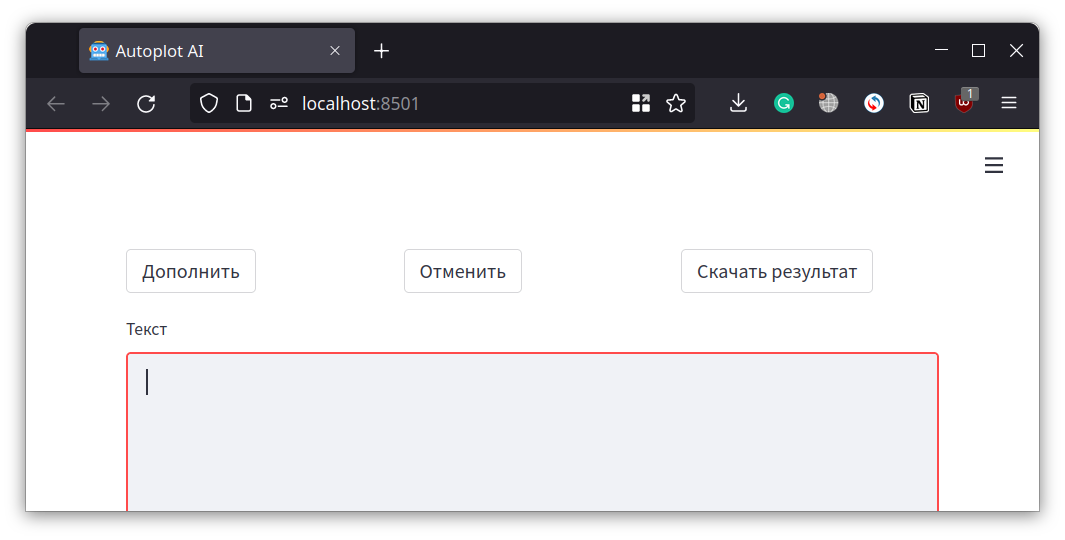
\includegraphics[width=\textwidth]{../inc/images/gui.png}
    \caption{Графический пользовательский интерфейс}
    \label{fig:gui}
\end{figure}

\section{Процесс работы с приложением}

Рассмотрим сценарий работы с приложением:
\begin{enumerate}
    \item пользователь вводит затравку (рисунок \ref*{fig:demo-0}),
    \item модель её продолжает (рисунок \ref*{fig:demo-1}),
    \item пользователь вводит дополнительную информацию, чтобы напрвить ход повествования (рисунок \ref*{fig:demo-2}),
    \item модель продолжает текст (рисунок \ref*{fig:demo-3}),
    \item пользователь остаётся неудовлетворён результатом, исправляет его и добавляет новые сведения (рисунок \ref*{fig:demo-4}).
\end{enumerate}

И в результате ещё нескольких итераций подобного процесса получается текст, показанный на рисунке \ref*{fig:demo-5}.

\begin{figure}
    \centering
    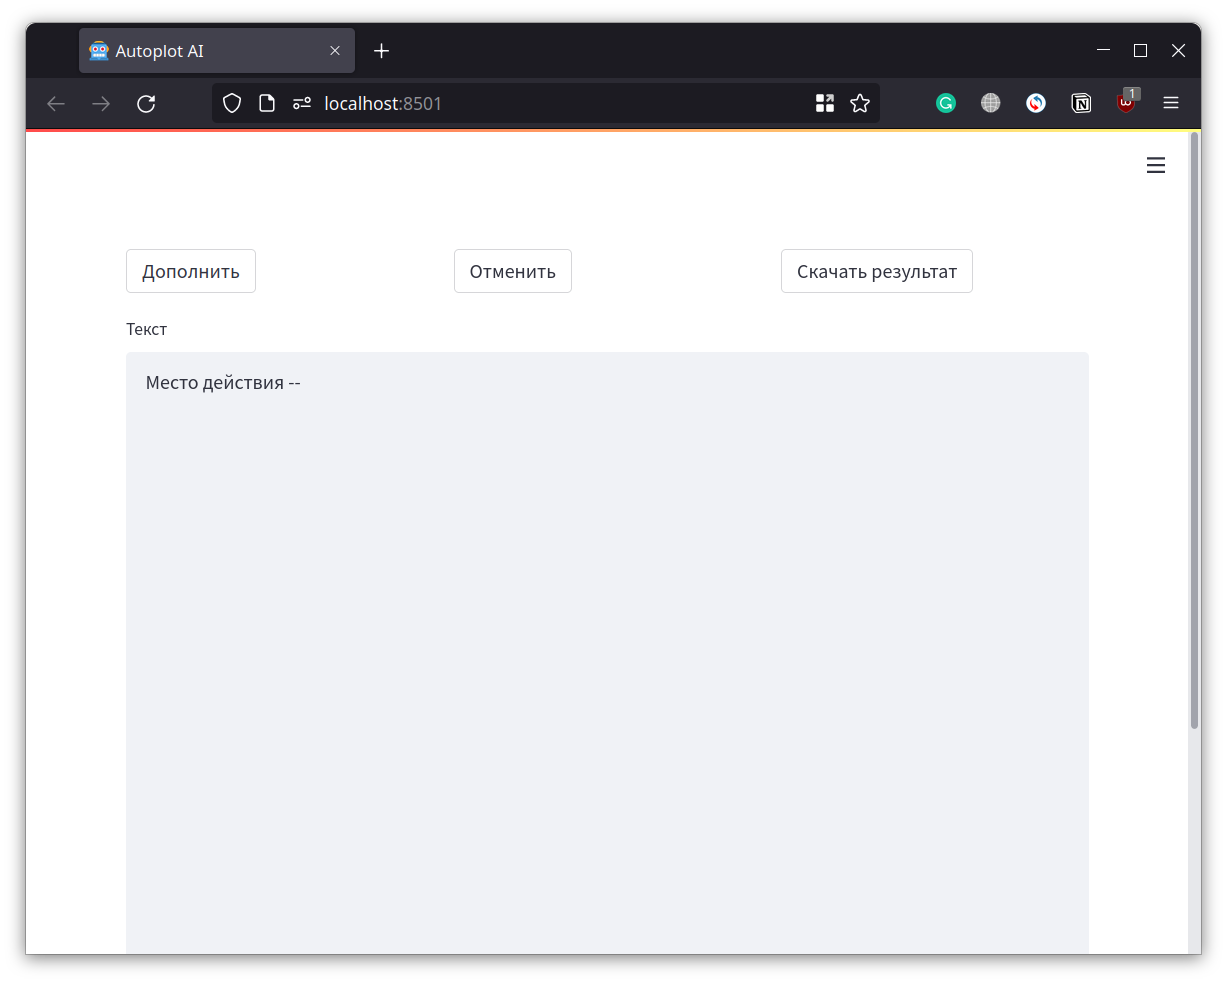
\includegraphics[width=0.8\textwidth]{../inc/images/demo-0.png}
    \caption{Ввод затравки}
    \label{fig:demo-0}
\end{figure}
\begin{figure}
    \centering
    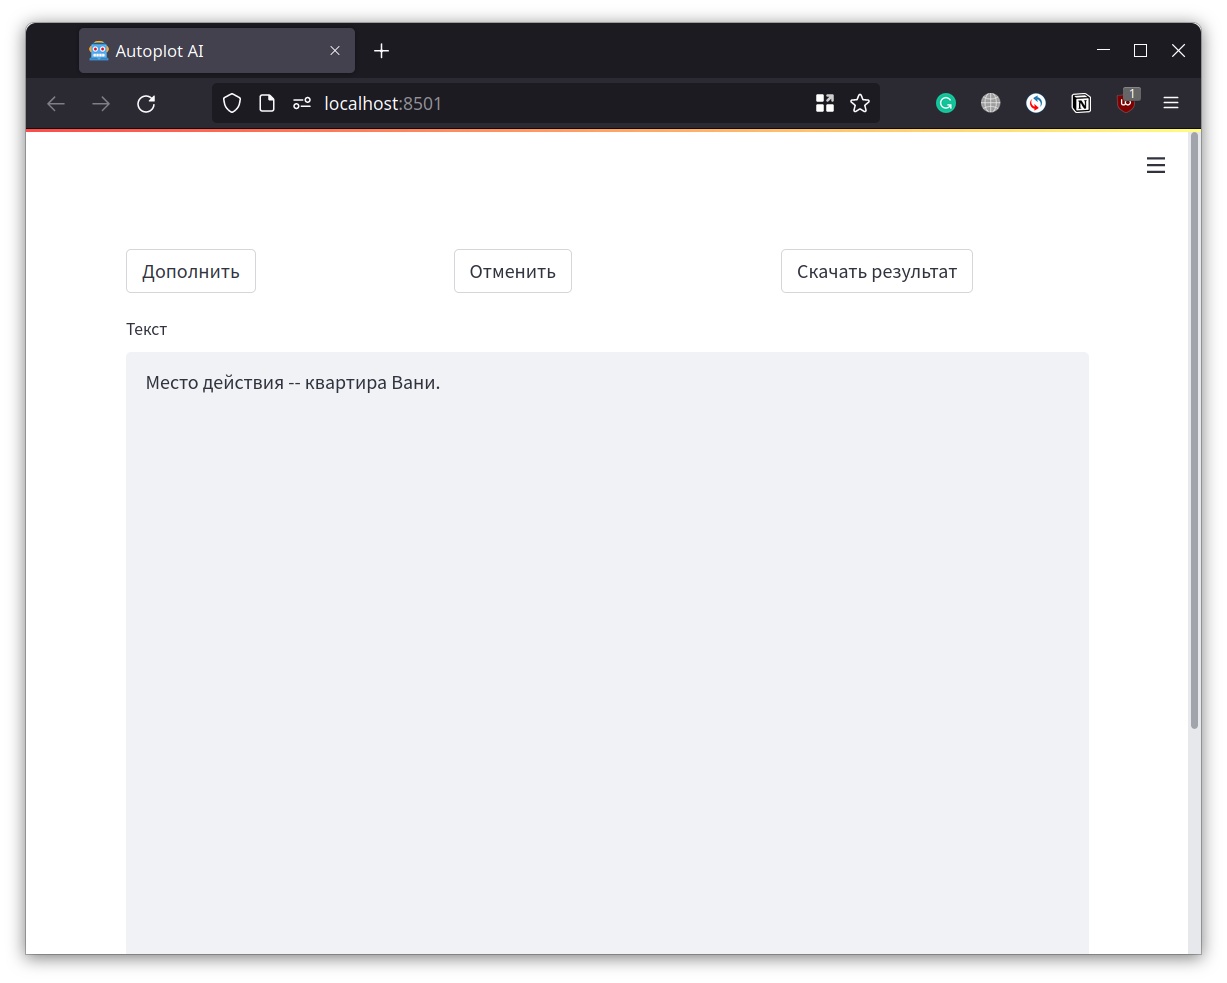
\includegraphics[width=0.8\textwidth]{../inc/images/demo-1.png}
    \caption{Дополнение затравки}
    \label{fig:demo-1}
\end{figure}
\begin{figure}
    \centering
    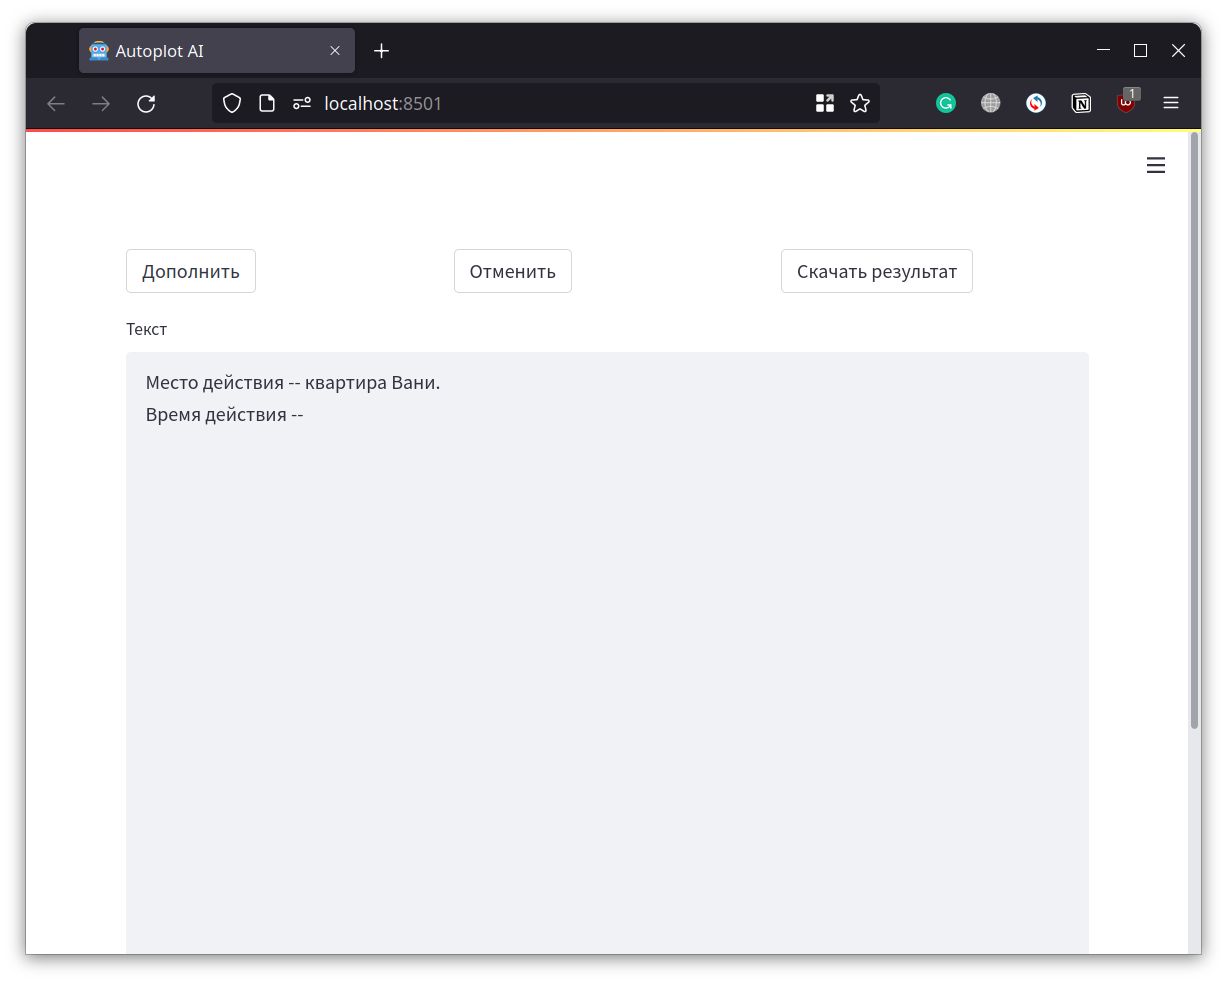
\includegraphics[width=0.8\textwidth]{../inc/images/demo-2.png}
    \caption{Ввод дополнительной информации}
    \label{fig:demo-2}
\end{figure}
\begin{figure}
    \centering
    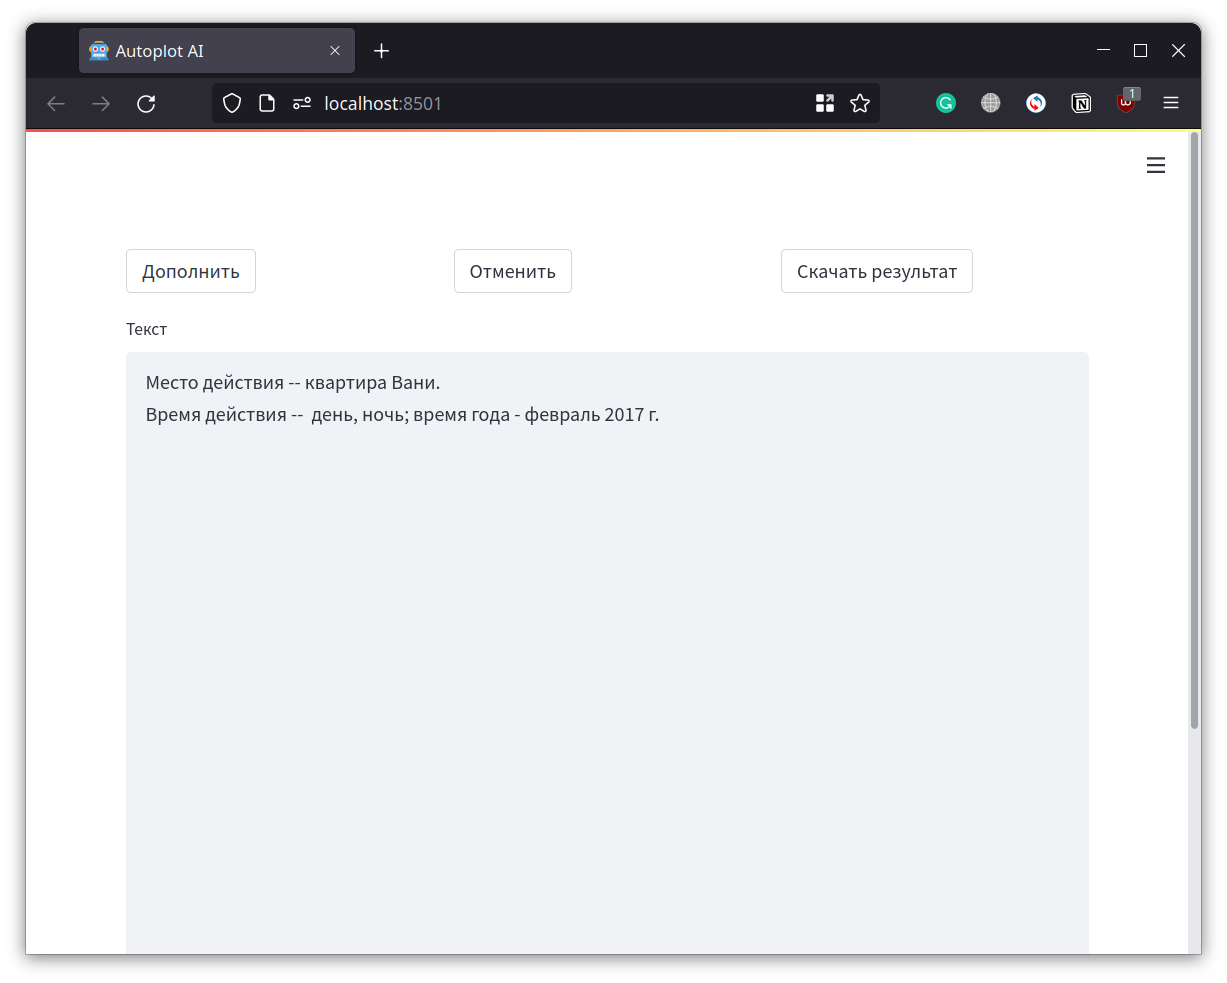
\includegraphics[width=0.8\textwidth]{../inc/images/demo-3.png}
    \caption{Генерация продолжения}
    \label{fig:demo-3}
\end{figure}
\begin{figure}
    \centering
    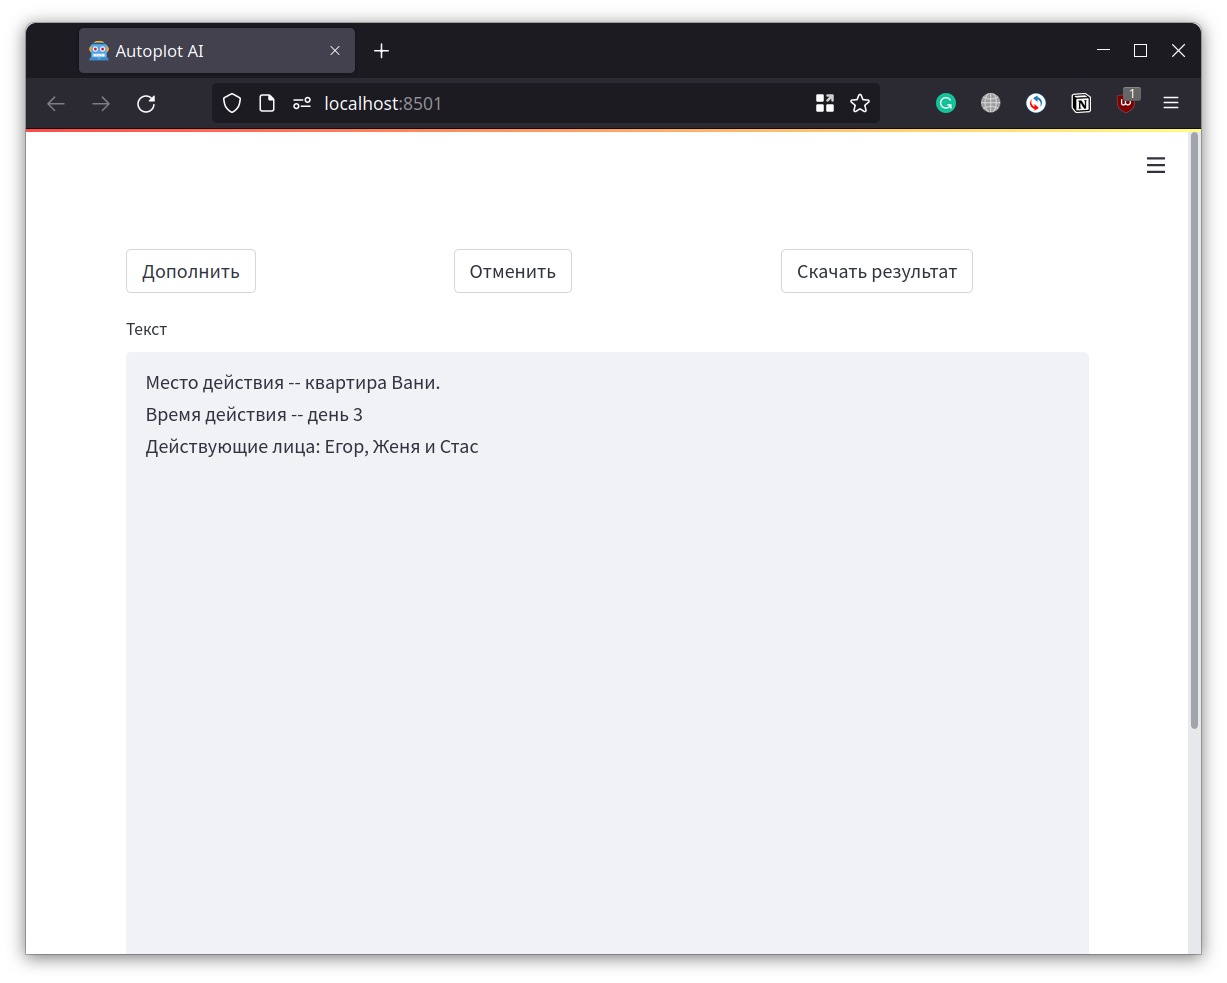
\includegraphics[width=0.8\textwidth]{../inc/images/demo-4.png}
    \caption{Исправление и ввод новой информации}
    \label{fig:demo-4}
\end{figure}
\begin{figure}
    \centering
    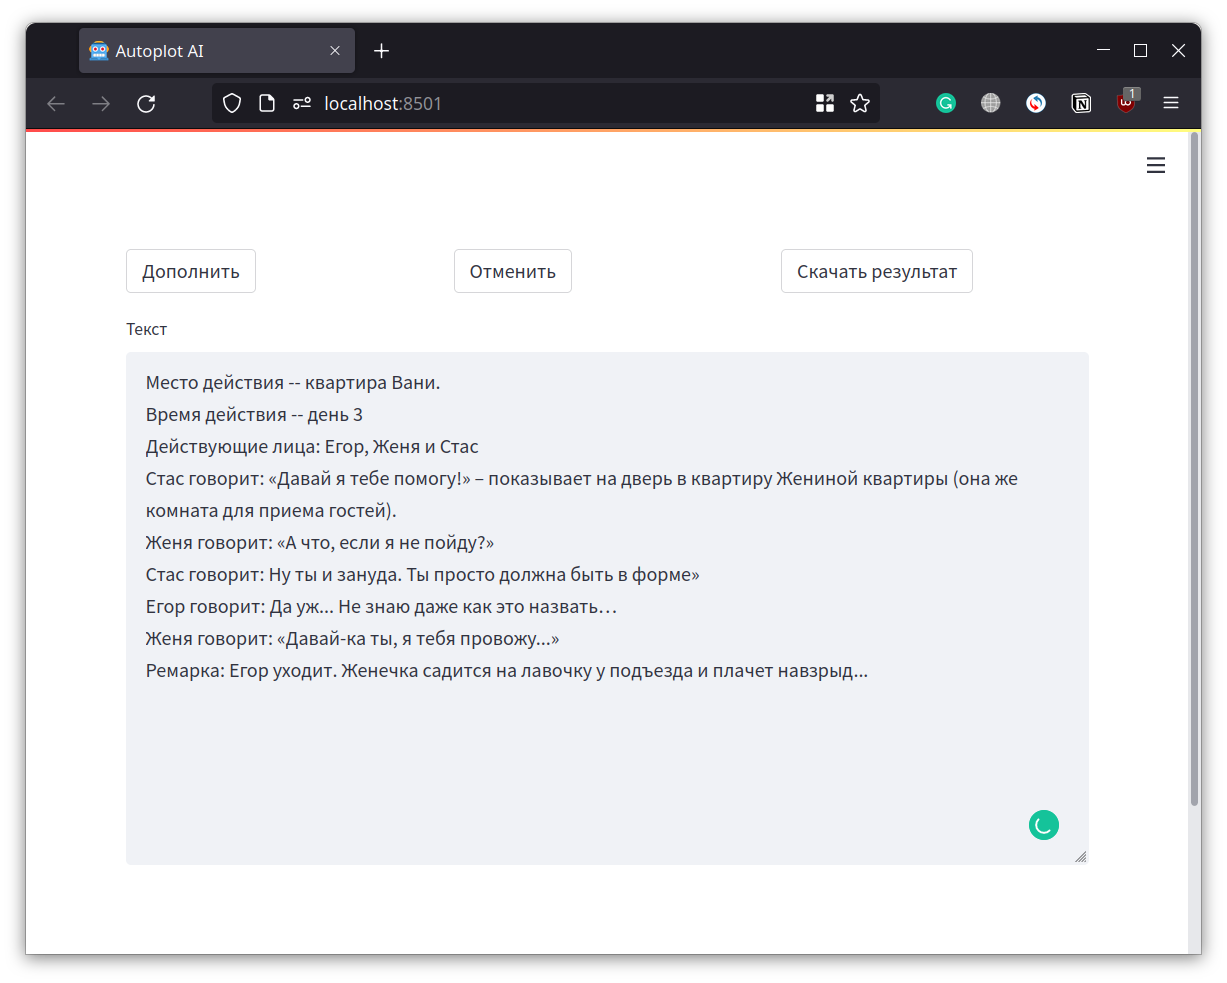
\includegraphics[width=0.8\textwidth]{../inc/images/demo-5.png}
    \caption{Результат генерации}
    \label{fig:demo-5}
\end{figure}

\section{Дистрибутив}

Для обеспечения переносимости и удобства распространения приложения все его файлы требуется поместить в один пакет и прописать инструкции по настройке и запуску программы.

Для выполнения этих требований была выбрана технология Docker. С её помощью всё, что необходимо программе для работы, а именно: исходный код, файлы модели, интерпретатор Python и библиотеки, помещаются в изолированное окружение, называемое контейнером и представляющее собой виртуальную машину с облегчённой операционной системой Debian \cite{doc:docker}.

В таком виде для передачи программы пользователю достаточно предоставить один файл --- Docker-образ, который он сможет запустить с помощью всего одной команды \verb|docker-compose up --build|.

\lstinputlisting[caption={Главный скрипт \Code{Dockerfile}}, label=lst:dockerfile]{../inc/code/Dockerfile.txt}
\lstinputlisting[caption={Compose-файл}, label=lst:docker-compose]{../inc/code/docker-compose.yml}

\Code{Dockerfile} (листинг \ref*{lst:dockerfile}) отвечает за сборку образа. Он настраивает Python-окружение, скачивает зависимости и файл модели. Compose-файл (листинг \ref*{lst:docker-compose}) нужен для упрощения процедуры запуска. Так как это веб-приложение, нужно знать адрес и порт, чтобы его открыть, и compose-файл производит связывание внутреннего порта Docker-контейнера с внешним на компьютере пользователя. Таким образом, страница с веб-приложением всегда располагается по адресу http://localhost:8501.